
\chapter{The ``software crisis'' and encapsulation}

This book is going to dive deeply into a huge pile of nuts and bolts. But
before we take the leap into particulars, it's important to stand briefly at
the precipice and understand why we're jumping. What does ``object-oriented''
mean? What problem was it intended to solve? When was it invented and why?

\section{Ancient history}

A long time ago, in our own galaxy, a situation emerged which has been labeled
\textbf{the software crisis}. This crisis didn't happen at an instant in time;
it was a set of disagreeable circumstances which gradually evolved until it
became unbearable. The crisis is usually dated somewhere in the 1970's. This
was just as the high-tech computing industry was really starting to heat up,
on its way to permanently changing the lives of almost everyone on the planet.

Now ``crisis'' is an alarming word, designed to get your attention. It's worth
asking what all the hubbub was about. The immediate symptom may not strike you
as a three-alarm fire: it was simply that software projects were tending to
overrun their schedules.

The '70's were not a very plug-and-play era, since standards had not yet
evolved to facilitate intercompatibilities between devices or programs. So the
focus was often on building complete systems from the ground up. Engineering
teams would plan releases of key product lines that involved numerous
components, such as system architecture, hardware design and integration, data
collection and organization, system and network configuration, and software
development at both the operating system and the end user levels.

What managers discovered was that consistently, the \textit{software}
components of projects were coming in late and over-budget. Sometimes, they
didn't get finished at all. When they did, they were buggy and brittle. And
they were especially vulnerable to requirements changes: if circumstances were
discovered during the project that required a change in the way the software
needed to work, the software team was often strikingly unable to adapt to
this. They could be set back weeks or months to implement even a modest
change.

This astonished everyone at the time. After all, ``\textit{soft}ware'' -- a
pun on ``hardware'' -- was a term intended to convey the flexible, malleable
nature of computer programs as contrasted with physical devices. Software was
supposed to be easy to write and easy to change. That was the point. You
didn't need complex manufacturing processes: you needed a desktop computer and
a text editor. And you (seemingly) didn't face challenges of scale the way you
did with hardware: you could run out of room to put logic circuits on a chip
or a motherboard, but there was no limit to the size of a text file. 

So building complex stuff quickly, and turning on a dime when necessary, ought
to be easy to do in software. Right?

\subsection{Quantifying the crisis}

I've never seen any hard data quantifying the budget overruns and delays that
software projects faced in the 1970's. It's possible to sketch it
conceptually, though. Take a look at Figure~\ref{fig:complexityCurve}. This is
my attempt to show the main dynamic at work.

\begin{figure}[ht]
\centering
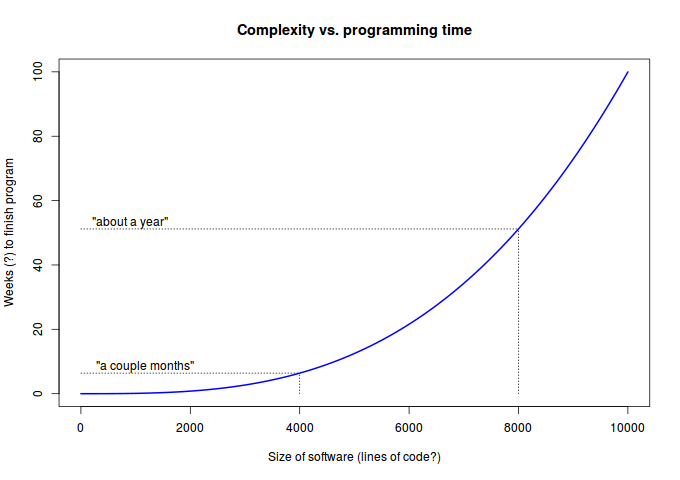
\includegraphics[width=0.9\textwidth]{complexityCurve.png}
\caption{The software crisis quantified: how long it took to complete a
program of various sizes. (Conceptual.)}
\label{fig:complexityCurve}
\end{figure}

On the $x$-axis is some measure of the \textit{complexity} of a proposed
computer program. Now complexity is devilishly difficult to quantify --
\textit{League of Legends} is more complex than \textit{Angry Birds}, but by
how much? Twice as complex? Ten times? A hundred times? I'll have a better
answer to that in a few paragraphs, but for now, as a proxy we'll just use the
\textit{size} of the program, measured in \textbf{lines of code}\footnote{I
know what you're thinking, and you're right. Not all lines of code are equally
complex. Some of them are just variable assignments, whereas others are parts
of complicated loops or function calls. Heck, some are just comments. Heck,
some are actually \textit{blank}. While all true, this analysis is conceptual
anyway, and we can surely say that raw program length is at least
\textit{somewhat} related to complexity -- show me a real-life ten-line
program that's actually more complex than a real-life ten-thousand-line
program and I'll concede.\\By the way, ``lines of code'' is sometimes
abbreviated ``LOC.'' Even more common is the abbreviation ``KLOC'' for
``thousands of lines of code.''}.

On the $y$-axis is the corresponding amount of time it would take a
programming team of a certain size to design, build (code), and test the
program.\footnote{Note carefully that this has nothing to do with how long the
code takes to \textit{run}. We're talking about programmer-time here, not
CPU-time.} As with the $x$-axis, we're making all kinds of simplifying
assumptions here: we're not worrying about exactly how many developers
there are, how much experience they each have, what language they're writing
in, \textit{etc.} That's okay. The point of this exercise is simply to
recognize the nature of the curve, showing how these two fuzzy variables were
related in the '70's.

A daunting curve it is, too. And very counterintuitive to project managers.
One would assume that if a 4,000-line program took the development team a
couple of months to release, an 8,000-line program would take about twice that
long. After all, it's twice as many lines, right?

The reality was not even close. A program with twice as many lines could
easily take \textit{four} times as long to build...or six, or ten, or twenty.
Worse, the programs that were built were also very hard to \textit{change}.
Take a large enough program and try to add a feature, fix a bug, or support a
new data format, and you inevitably broke something else while making the
change. Then you fixed what you broke, but \textit{d'oh!!} broke something
else by doing so, \textit{etc.}

It was miserable, especially because advances in other areas (like hardware)
were making exciting technologies possible for the first time. Everyone was
rarin' to go, yet unexpectedly the software (supposedly the easy part) was
gumming up the works.

For a time, it almost seemed as if the human race had uncovered some built-in
limitation of the universe, like the speed of light. This hypothetical limit
might have been called ``maximum complexity,'' meaning the greatest amount of
sophistication one could build in to a single logical creation. That curve in
Figure~\ref{fig:complexityCurve} starts to go up fast. Maybe, people
depressingly thought, a functioning 200,000-line program isn't even
\textit{possible} to create? That threatened to put a damper on a lot of
expectations.

\section{Software and complexity}

% The software crisis

% "soft"ware
% time vs. complexity curve

% Programming language diagram

\section{Dependencies}

\section{Encapsulation}

\section{Features of OO}

% \section{Exercises}
% 
% Use an index card or a piece of paper folded lengthwise, and cover up the
% right-hand column of the exercises below. Read each exercise in the
% left-hand column, answer it in your mind, then slide the index card down to
% reveal the answer and see if you're right! For every exercise you missed,
% figure out why you missed it before moving on.
% 
% \begin{small}
% \begin{enumerate}
% \newcolumntype{Q}{>{\arraybackslash}m{.3\textwidth}}
% \newcolumntype{A}{>{\arraybackslash}m{.6\textwidth}}
% %\begin{longtable}{m{0.3\textwidth} || m{0.6\textwidth}}
% \begin{longtable}{Q || A}
% \hline
% \item 
% What key software problem was the OO paradigm invented to address?
% &
% Too many dependencies.
% \\
% \hline
% 
% \end{longtable}
% \end{enumerate}
% \end{small}
